\documentclass[pdftex,12pt,a4paper]{article}

\usepackage{graphicx}  
\usepackage[margin=2.5cm]{geometry}
\usepackage{breakcites}
\usepackage{indentfirst}
\usepackage{pgfgantt}
\usepackage{pdflscape}
\usepackage{float}
\usepackage{epsfig}
\usepackage{epstopdf}
\usepackage[cmex10]{amsmath}
\usepackage{stfloats}
\usepackage{multirow}
\graphicspath{{./images/}}
\usepackage{tikz-timing}

\renewcommand{\refname}{REFERENCES}
\linespread{1.3}

\usepackage{mathtools}
%\newcommand{\HRule}{\rule{\linewidth}{0.5mm}}
\thispagestyle{empty}
\begin{document}
\begin{titlepage}
\begin{center}
\textbf{}\\
\textbf{\Large{ISTANBUL TECHNICAL UNIVERSITY}}\\
\vspace{0.5cm}
\textbf{\Large{COMPUTER ENGINEERING DEPARTMENT}}\\
\vspace{2cm}
\textbf{\Large{BLG 242E\\ DIGITAL CIRCUITS LABORATORY\\ HOMEWORK REPORT}}\\
\vspace{2.8cm}
\begin{table}[ht]
\centering
\Large{
\begin{tabular}{lcl}
\textbf{HOMEWORK NO}  & : & 3 \\
\textbf{LAB SESSION}  & : & FRIDAY - 16.30 \\
\textbf{GROUP NO}  & : & 18 \\
\end{tabular}}
\end{table}
\vspace{1cm}
\textbf{\Large{GROUP MEMBERS:}}\\
\begin{table}[ht]
\centering
\Large{
\begin{tabular}{rcl}
150200916  & : & Denıs Iurıe Davıdoglu \\
150220770  & : & Onur Baylam \\
\end{tabular}}
\end{table}
\vspace{2.8cm}
\textbf{\Large{SPRING 2023}}

\end{center}

\end{titlepage}

\thispagestyle{empty}
\addtocontents{toc}{\contentsline {section}{\numberline {}FRONT COVER}{}}
\addtocontents{toc}{\contentsline {section}{\numberline {}CONTENTS}{}}
\setcounter{tocdepth}{4}
\tableofcontents
\clearpage

\setcounter{page}{1}

\section{INTRODUCTION}

In this homework, three-state logic is explored for designing data buses and basic memory. Along low and high states, a net can also get high impedance state, which behaves as if not connected to the circuit at all. By connecting a zero or an one to high impedance wire, there is no risk of creating short circuit, and the wire gets the same voltage as the connected input. This allows turning outputs of a logic circuit on and off, and connecting many three-state units to a common bus.

\section{MATERIALS, METHODS AND RESULTS}
\subsection{Part 1}
Before starting with the first part, the most basic component of three-state logic, the buffer, is designed. Buffers can be inverting and non-inverting, and with the goal of transmitting data to a bus, non-inverting type is considered. There are two inputs and one output; if enable input is low, output should be high impedance state, otherwise output will be equal to input data. Using a continuous assignment with ternary operator in Verilog, buffer is implemented and simulated:
\begin{figure}[H]
\centering
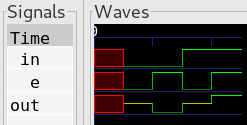
\includegraphics[width=0.7\textwidth]{buffer_wave.png}
\caption{3-state buffer simulation}
\end{figure}

Next, to test the capability of designed buffer to form a bus, the following circuit is tested:

\begin{figure}[H]
\centering
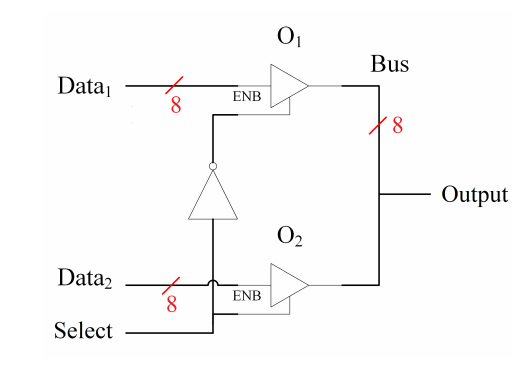
\includegraphics[width=\textwidth]{part1_original.png}
\caption{8-bit data bus with 2 drivers with 3-state buffers}
\end{figure}

\begin{figure}[H]
\centering
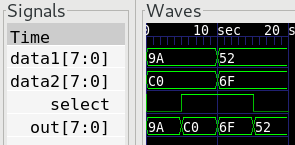
\includegraphics[width=0.7\textwidth]{part1_wave.png}
\caption{Part 1's simulation}
\end{figure}

As it is seen from simulation, we are capable of multiplexing data using select input, without actually using a multiplexer.

\subsection{Part 2}
Buses are supposed to not only be written to, but also read from. By extending the module from previous part, two controlled outputs can be added, as in the diagram:

\begin{figure}[H]
\centering
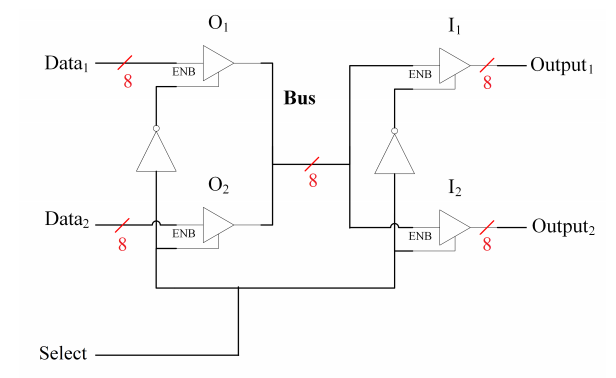
\includegraphics[width=\textwidth]{part2_original.png}
\caption{8-bit data bus with 2 drivers and 2 readers}
\end{figure}

The behaviour of the outputs in this module slightly differs from the previous module. While the bus gets the same data, we do not pay attention to it anymore, and instead focus on the controlled outputs. When an output is not selected, it enters high impedance state:

\begin{figure}[H]
\centering
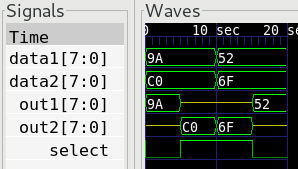
\includegraphics[width=0.7\textwidth]{part2_wave.png}
\caption{Part 2's simulation}
\end{figure}

\subsection{Part 3}
Here an 8-bit memory line module is explained. In order to use registers on a common bus, their outputs should be tri-stated using buffers. They should have write enable and read enable inputs, and normally these will not be active both at the same time, because the both are meant to be connected to bus. Module has a positive edge triggered clock for loading data and a negative edge triggered reset. Outputting internal data is done asynchronously, and the advantage is that in a real-world application, data should be already stabilized on the bus upon being read.

\begin{figure}[H]
\centering
\begin{tabular}{|c|c|c|c|c||c|c|}
	\hline
	 Clock & Reset & LineSel & Write & Read & Data & Output \\
	\hline
	\texttiming{LH} & $\phi$ & 1 & 1 & $\phi$ & Input & ? \\
	$\phi$ & \texttiming{HL} & $\phi$ & $\phi$ & $\phi$ & 0 & ? \\
	$\phi$ & $\phi$ & 1 & $\phi$ & 1 & ? & Data \\
	$\phi$ & $\phi$ & 0 & $\phi$ & 1 & ? & Z \\
	$\phi$ & $\phi$ & 1 & $\phi$ & 0 & ? & Z \\
	$\phi$ & $\phi$ & 0 & $\phi$ & 0 & ? & Z \\
	\hline
\end{tabular}
\caption{8-bit memory line's truth table}
\end{figure}

\begin{figure}[H]
\centering
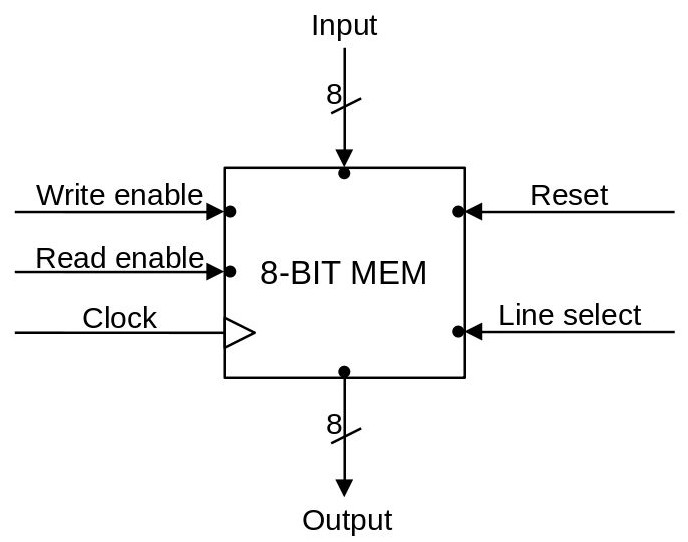
\includegraphics[width=0.7\textwidth]{part3_diagram.jpg}
\caption{8-bit memory line module}
\end{figure}

Memory line module's simulation results corresponds to the function table:

\begin{figure}[H]
\centering
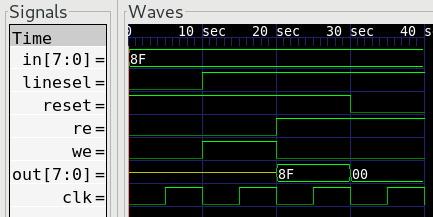
\includegraphics[width=0.7\textwidth]{part3_wave.png}
\caption{Part 3's simulation}
\end{figure}

\subsection{Part 4}
Many 8-bit memories can be arranged to form an 8-byte memory. Input, clock, reset, read enable and write enable are common for all of 8-bit memories, and to perform individual read and write operations, line selects are utilized. 8-bit memory has extra 3-bit adress input and chip select, which ramify through a decoder to enable small memories one at a time:
\begin{figure}[H]
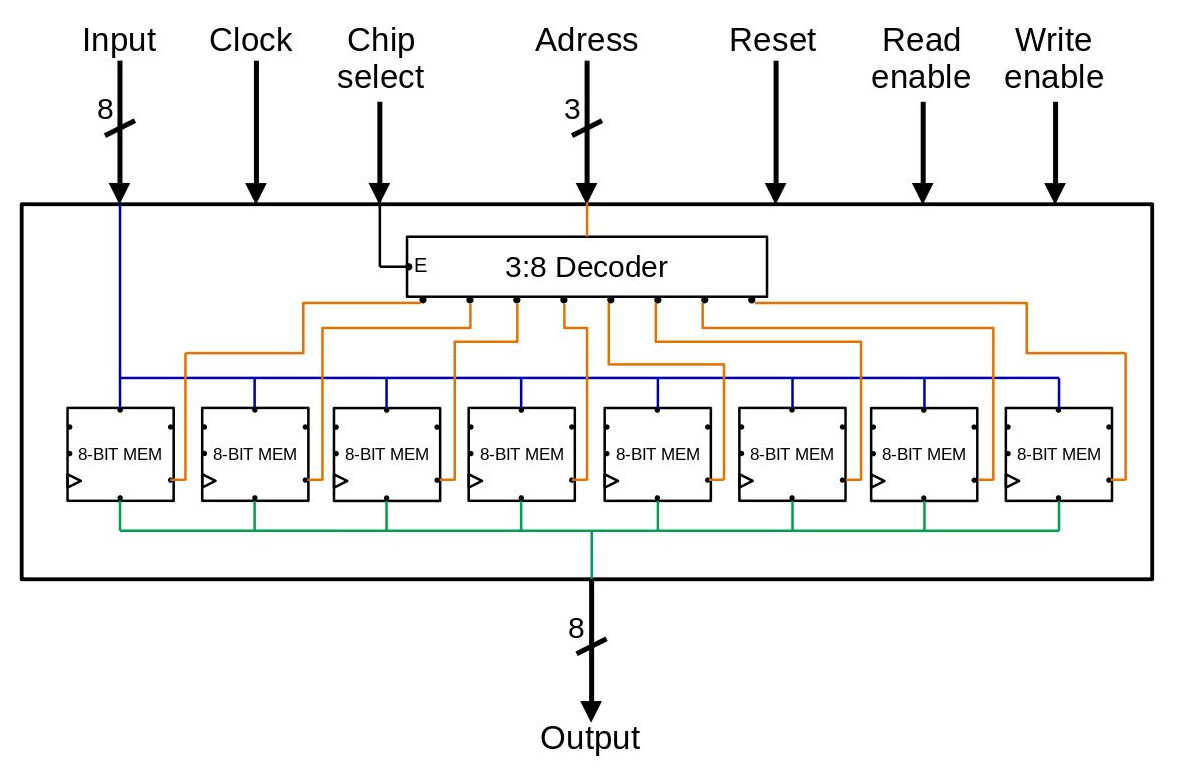
\includegraphics[width=\textwidth]{part4_diagram.jpg}
\caption{8-byte memory using 8-bit memory line modules}
\end{figure}

Testbench for this memory checks the correctness of load, output and clear operations:

\begin{figure}[H]
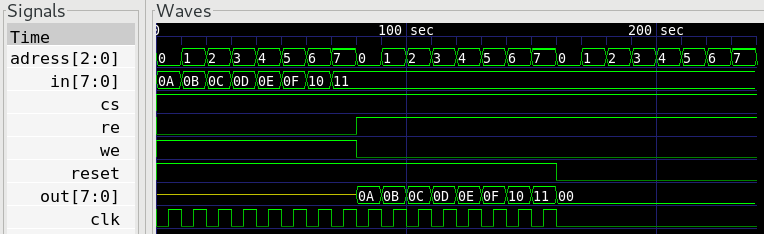
\includegraphics[width=\textwidth]{part4_wave.png}
\caption{Part 4's simulation}
\end{figure}

\subsection{Part 5}
\subsection{Part 6}

\section{CONCLUSION}
Comment on any difficulties you have faced, what you have learned etc.


\end{document}

